\documentclass[12pt]{article}
\usepackage[margin=2.5cm]{geometry}
\usepackage{enumerate}
\usepackage{amsfonts}
\usepackage{amsmath}
\usepackage{fancyhdr}
\usepackage{amsmath}
\usepackage{amssymb}
\usepackage{amsthm}
\usepackage{mdframed}
\usepackage{graphicx}
\usepackage{subcaption}
\usepackage{adjustbox}
\usepackage{listings}
\usepackage{xcolor}
\usepackage{courier}
\usepackage[utf]{kotex}
\usepackage{hyperref}

\definecolor{codegreen}{rgb}{0,0.6,0}
\definecolor{codegray}{rgb}{0.5,0.5,0.5}
\definecolor{codepurple}{rgb}{0.58,0,0.82}
\definecolor{backcolour}{rgb}{0.95,0.95,0.92}

\lstdefinestyle{mystyle}{
    backgroundcolor=\color{backcolour},
    commentstyle=\color{codegreen},
    keywordstyle=\color{magenta},
    numberstyle=\tiny\color{codegray},
    stringstyle=\color{codepurple},
    basicstyle=\ttfamily\footnotesize,
    breakatwhitespace=false,
    breaklines=true,
    captionpos=b,
    keepspaces=true,
    numbers=left,
    numbersep=5pt,
    showspaces=false,
    showstringspaces=false,
    showtabs=false,
    tabsize=1
}

\lstset{style=mystyle}

\pagestyle{fancy}
\renewcommand{\headrulewidth}{0.4pt}
\lhead{CSC 369}
\rhead{Worksheet 1 Solution}

\begin{document}
\title{CSC 369 Worksheet 1 Solution}

\maketitle

\bigskip

\begin{enumerate}[1.]
    \item

    \bigskip

    The cpu utilization is 100\%.

    \bigskip

    The CPU utilization formula is given as

    \begin{align}
        \text{CPU Utilization} &= 1 - \prod\limits_{i} \text{ I/O blocked time of ith process}
    \end{align}

    \bigskip

    Since the processes do no I/O, we can write there is no I/O blocked time.

    \bigskip

    Thus, we can conclude


    \begin{align}
        \text{CPU Utilization} &= 1 - 0\\
        &= 1
    \end{align}

    which is 100\%.

    \bigskip

    \underline{\textbf{Notes}}

    \begin{itemize}
        \item \textbf{CPU Utilization}

        \begin{itemize}
            \item Means \% of time CPU is in use
            \item Formula is

            \begin{align}
                \text{CPU Utilization} &= 1 - \prod\limits_{i} \text{ I/O blocked time of ith process}
            \end{align}
        \end{itemize}
        \item \textbf{Process}

        \begin{itemize}
            \item Means a program in execution
        \end{itemize}

        \item \textbf{PID}

        \begin{itemize}
            \item Is a short hand form for `process identifier'
        \end{itemize}

        \item \textbf{Process States}

        \begin{itemize}
            \item in simplified view, process can be in one of the three states

            \begin{enumerate}[1.]
                \item \textbf{Running:}
                \begin{itemize}
                    \item Is running on a processor
                    \item Means `Is executing instructions'
                \end{itemize}
                \item \textbf{Ready:}

                \begin{itemize}
                    \item Is ready to run
                    \item But, OS chosen to not to run it at the moment
                \end{itemize}
                \item \textbf{Blocked:}

                \begin{itemize}
                    \item Is not ready to run until some other event takes place

                    \bigskip

                    \underline{\textbf{Example}}

                    Running an I/O request to disk $\to$ process blocked $\to$ other process can do their job while waiting
                \end{itemize}
            \end{enumerate}
        \end{itemize}
    \end{itemize}

    \item

    It takes total of 10 seconds to run.

    \bigskip

    The first task only uses CPU, and takes 4 seconds.

    \bigskip

    But, for the second task, on top of 4 seconds used for I/O, 1 second is used for preparing and initiating I/O,
    and the other 1 second is used for signaling that I/O is done.

    \bigskip

    So in total, we have $4 + 4 + 1 + 1 = 10$ seconds.

    \begin{center}
    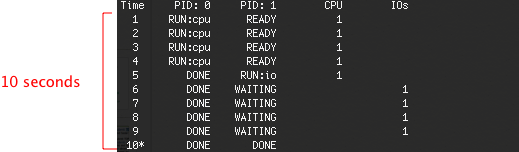
\includegraphics[width=\linewidth]{images/worksheet_1_solution_1.png}
    \end{center}

    \item

    Yes. Switching the order does matter.

    \bigskip

    When the order is switched, the process 2 with I/O runs, and the process 2 enters
    the blocked state.

    \bigskip

    While at blocked state, the other process executes.

    \bigskip

    Since both take 4 seconds, by the time process 2 finishes, process 1 is finished.

    \bigskip

    Thus, total of 6 seconds are taken.

    \item

    With flag SWITCH\_ON\_END, system runs as if it's without I/O. That is,
    process 2 runs after process 1 finishes.

    \bigskip

    The only difference is that process 2 executes at the same time process 1 finishes.

    \bigskip

    So instead of 10 seconds, there are 9 seconds in total

    \begin{center}
    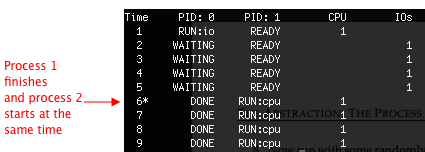
\includegraphics[width=\linewidth]{images/worksheet_1_solution_2.png}
    \end{center}

    \item

    I need to write what happens when one is waiting for I/O (SWITCH\_ON\_IO).

    \bigskip

    The result is the same as question 2.

    \bigskip

    While process 1 is in blocked state, process 2 is executes.

    \begin{center}
    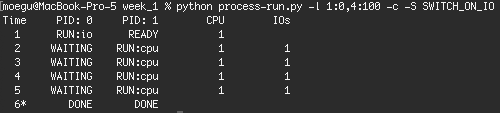
\includegraphics[width=\linewidth]{images/worksheet_1_solution_3.png}
    \end{center}

    \item

    First, I need to write what happens when combination of processes (-I IO\_RUN\_LATER, SWITCH\_ON\_IO) are used.

    \bigskip

    There are total of four processes.

    \bigskip

    While process 1 is in blocked state for I/O, process 2 executes.

    \bigskip

    When process 1 finishes its first I/O operation, it doesn't execute the next right away. It waits for process 3 and 4
    to finish until it finally gets its turn for more I/O operations.

    \bigskip

    Second, I need to write if the system resources are effectively utilized uder the combination of processes.

    \bigskip

    The answer is no.

    \bigskip

    System resources could have been utilized more effectively if process 3 and 4
    are run while process 1 is performing it's I/O operation.

    \begin{center}
    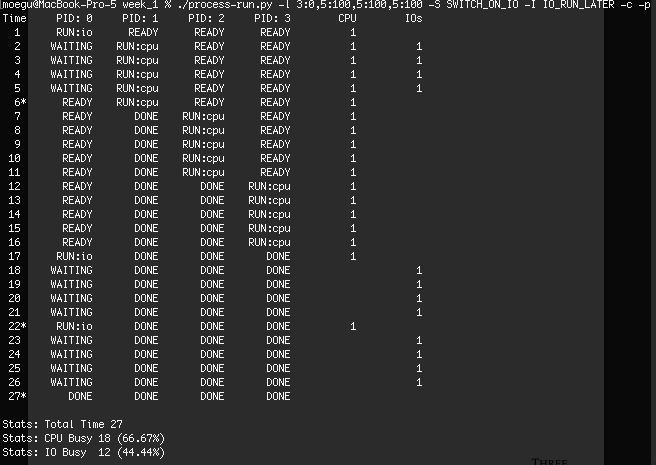
\includegraphics[width=\linewidth]{images/worksheet_1_solution_4.png}
    \end{center}

    \item

    First, I need to write the difference between the process with \texttt{-I IO\_RUN\_LATER}
    and \texttt{-I IO\_RUN\_IMMEDIATE}.

    \bigskip

    When the process is run with \texttt{-I IO\_RUN\_IMMEDIATE}, process 1 runs immediately one after another.
    And in each of process 1's blocked state, other processes are executed (process 2, process 3, process 4).

    \bigskip

    This differs from \texttt{-I IO\_RUN\_LATER} where process 1
    waits until other processes finish.

    \bigskip

    \begin{center}
    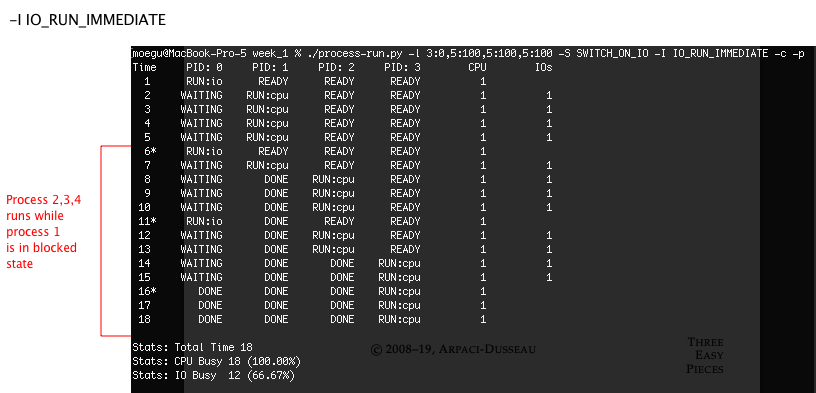
\includegraphics[width=\linewidth]{images/worksheet_1_solution_5.png}
    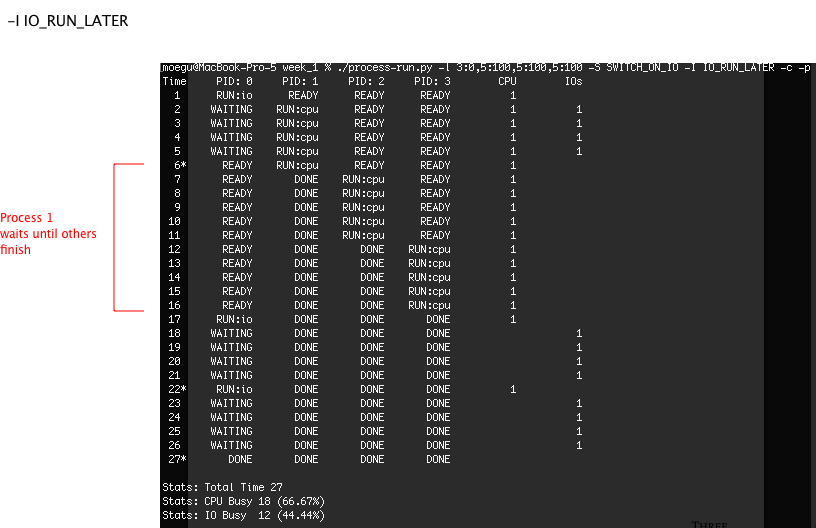
\includegraphics[width=\linewidth]{images/worksheet_1_solution_6.png}
    \end{center}

    Second, I need to write why running a process that just completed an I/O again is
    a good idea?

    \bigskip

    It is a good idea since processes are better managed. That is, more can be done
    in less amount of time.

    \item

    I need to write what happens when the following flags are used

    \begin{itemize}
        \item \texttt{-I IO\_RUN\_IMMEDIATE} vs \texttt{-I IO\_RUN\_LATER}

        \begin{itemize}
            \item \texttt{ -s 1 -l 3:50,3:50}

            \bigskip

            When it is run with \texttt{-I IO\_RUN\_IMMEDIATE}, the CPU part of process 1
            executes while process 2 waits in ready state.

            \bigskip

            When process 1 enters blocked state for I/O, process 2 starts.

            \bigskip

            We know that process 1 stays in blocked state for 4 seconds for each I/O operation.

            \bigskip

            Since process 2 is all about CPU and takes 3 seconds to complete,
            process 2 will finish before process 1's second I/O operation.

            \bigskip

            Now, when it is run with \texttt{-I IO\_RUN\_LATER}, the same happens as above.

            \bigskip

            So, in this example, there is no difference between \texttt{-I IO\_RUN\_IMMEDIATE} and \texttt{-I IO\_RUN\_LATER}.

            \bigskip

            \begin{center}
            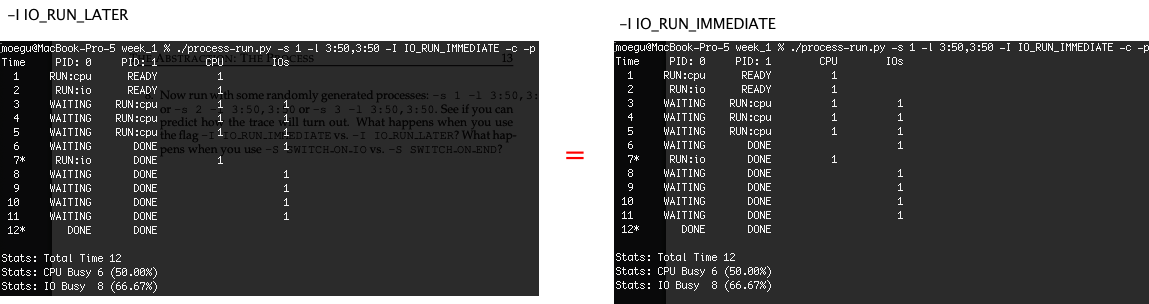
\includegraphics[width=\linewidth]{images/worksheet_1_solution_7.png}
            \end{center}

            \item \texttt{-s 2 -l 3:50,3:50}

            \bigskip

            When it is run with \texttt{-I IO\_RUN\_IMMEDIATE},
            process 1 enters blocked state for I/O operation at time = 2, and
            process 2 executes while process 1 is in blocked state between time = 2 and time = 5.

            \bigskip

            We know that each CPU operation takes 1 second and initialization of I/O operation takes 1 second.

            \bigskip

            Using this information, process 2 will enter blocked state for I/O operation at time = 3 until time = 6.

            \bigskip

            Then, at time = 6, process 1 will run another I/O operation and enter blocked state from time = 7 to time = 10.

            \bigskip

            Then, at time = 8, process 2 will run last I/O operation and enter blocked state from time = 9 to time = 12.

            \bigskip

            Then, at time = 11, process 1 will execute CPU operation, and will finish at the same time.

            \bigskip

            Now, when it is run with \texttt{-I IO\_RUN\_LATER}, the same happens as above.

            \bigskip

            So, in this example, there is no difference between \texttt{-I IO\_RUN\_IMMEDIATE} and \texttt{-I IO\_RUN\_LATER}.

            \begin{center}
            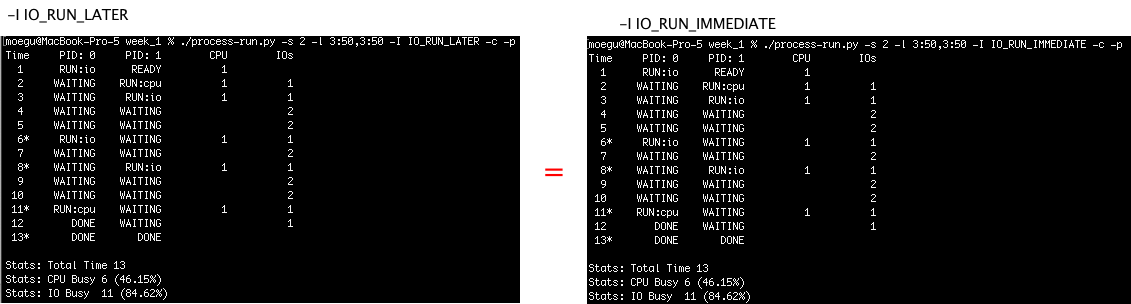
\includegraphics[width=\linewidth]{images/worksheet_1_solution_8.png}
            \end{center}

        \end{itemize}

        \item \texttt{-S SWITCH\_ON\_IO} vs \texttt{-S SWITCH\_ON\_END}

        \begin{itemize}
            \item \texttt{-s 3 -l 3:50,3:50}

            \bigskip

            When the processes are run with \texttt{-S SWITCH\_ON\_IO}, it will work the same as when ran with \texttt{-I IO\_RUN\_IMMEDIATE}.

            \bigskip

            However, when the processes are run with \texttt{-S SWITCH\_ON\_END}, process 2 will begin when
            process 1 finishes.

            \bigskip

            And this happens at time = 8.

            \bigskip

            \begin{center}
            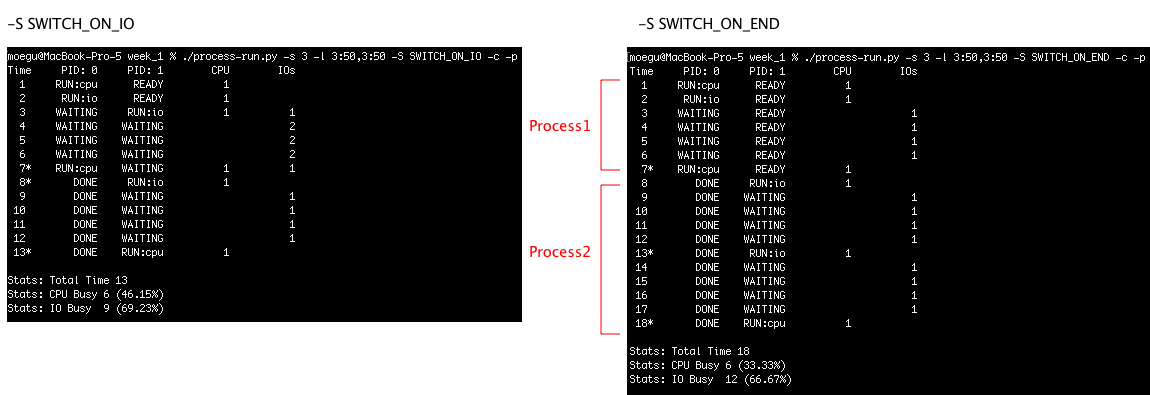
\includegraphics[width=\linewidth]{images/worksheet_1_solution_9.png}
            \end{center}

        \end{itemize}
    \end{itemize}

\end{enumerate}

\end{document}